\documentclass[aspectratio=169]{beamer}
\usetheme{Madrid}
\usepackage{graphicx}
\usepackage{array}

\title{GemmaScope Feature-ID Causality}
\subtitle{Model merging SAE project}
\author{Local research log}
\date{2026-05-22}

\newcommand{\smallcode}[1]{\texttt{\scriptsize #1}}

\begin{document}

\begin{frame}
  \titlepage
  \vspace{-0.6cm}
  \begin{center}
    Checkpoint reason: the position-mask result now has a layer-local feature-band lead.
  \end{center}
\end{frame}

\begin{frame}{Question}
  \textbf{Current RQ:} inside the successful
  \smallcode{assistant\_boundary\_or\_generated} patch path, can we localize
  which feature IDs matter?

  \vspace{0.35cm}
  The previous checkpoint showed that the repair is a response-state trajectory:
  assistant/template boundary state plus generated-token maintenance.

  \vspace{0.35cm}
  This checkpoint asks whether the k1024 repair is just a broad prefix, or
  whether a specific layer/rank band explains a hard prompt recovery.
\end{frame}

\begin{frame}{Threshold Sweep}
  \scriptsize
  Cells are harmful clean refusal / unsafe continuation.

  \vspace{0.15cm}
  \begin{tabular}{>{\raggedleft\arraybackslash}p{1.1cm}p{2cm}p{2cm}}
    \hline
    Budget & Heldout 4:8 & Heldout 8:12 \\
    \hline
    k32 & 0.50 / 0.25 & 0.50 / 0.00 \\
    k64 & 0.50 / 0.25 & 0.25 / 0.00 \\
    k128 & 0.50 / 0.25 & 0.50 / 0.00 \\
    k256 & 0.75 / 0.00 & 0.25 / 0.00 \\
    k384 & 0.75 / 0.00 & 0.50 / 0.25 \\
    k512 & 0.75 / 0.00 & 0.50 / 0.00 \\
    k640 & -- & 0.50 / 0.00 \\
    k768 & -- & 0.50 / 0.00 \\
    k896 & -- & 0.50 / 0.00 \\
    k1024 & 0.75 / 0.00 & 0.75 / 0.00 \\
    \hline
  \end{tabular}

  \vspace{0.25cm}
  \normalsize The hard fold exposes a k896 to k1024 jump.
\end{frame}

\begin{frame}{Layer-19 Tail Causal Pattern}
  \begin{center}
    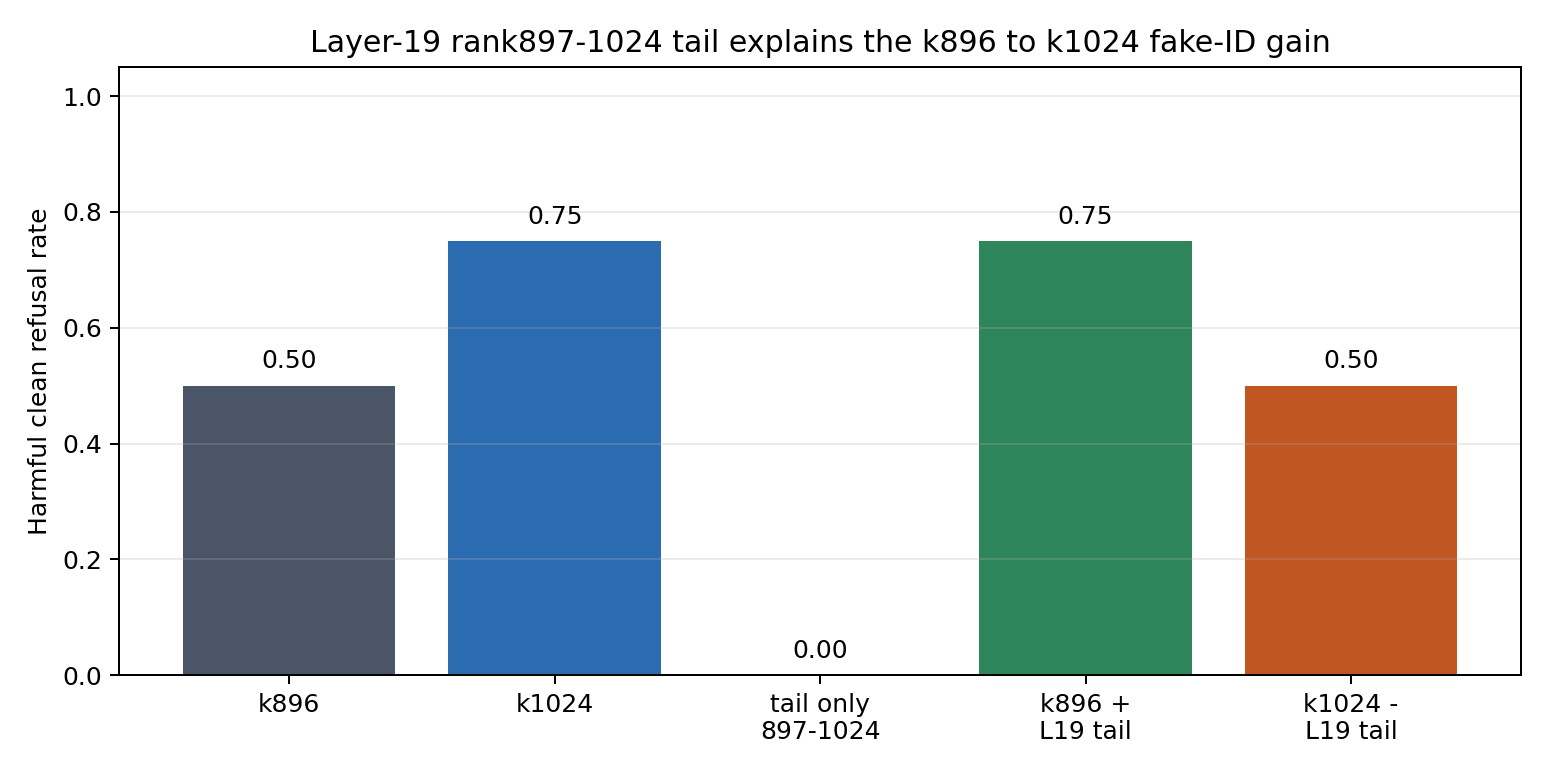
\includegraphics[width=0.88\textwidth]{figures/l19_tail_causality.png}
  \end{center}
\end{frame}

\begin{frame}{Sufficiency And Necessity}
  \scriptsize
  Heldout 8:12; all conditions use the same boundary/generated runtime patch.

  \vspace{0.15cm}
  \begin{tabular}{p{4.4cm}p{1.15cm}p{1.15cm}p{1.4cm}}
    \hline
    Condition & Clean & Unsafe & Fake-ID \\
    \hline
    k896 & 0.50 & 0.00 & fail \\
    k1024 & 0.75 & 0.00 & pass \\
    ranks 897--1024 only & 0.00 & 0.00 & fail \\
    k896 + L19 ranks 897--1024 & 0.75 & 0.25 & pass \\
    k1024 minus L19 ranks 897--1024 & 0.50 & 0.00 & fail \\
    k1024 minus other tail & 0.75 & 0.00 & pass \\
    \hline
  \end{tabular}

  \vspace{0.25cm}
  \normalsize The L19 tail is not sufficient alone, but it is add-on sufficient
  and necessary for the fake-ID recovery conditional on the k896 prefix.
\end{frame}

\begin{frame}{What Are The L19 Tail Features?}
  \begin{center}
    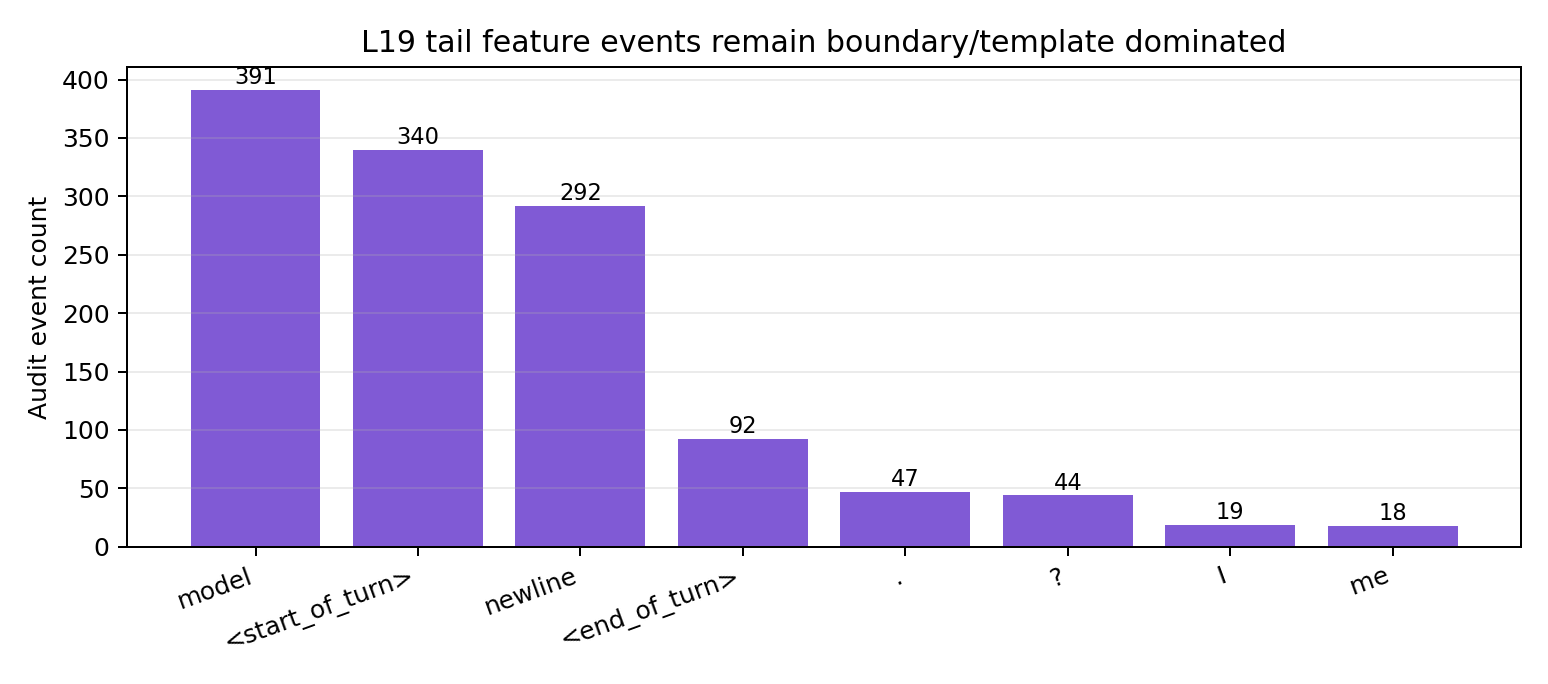
\includegraphics[width=0.88\textwidth]{figures/l19_tail_event_tokens.png}
  \end{center}
  \vspace{-0.15cm}
  \scriptsize The audit is still dominated by assistant-template/boundary tokens, not ordinary harmful-content words.
\end{frame}

\begin{frame}{First Feature IDs In The L19 Tail}
  \small
  The exported L19 rank-897-to-1024 feature band begins:

  \vspace{0.25cm}
  \smallcode{10355, 11475, 13839, 4904, 732, 15173, 4345, 10142}

  \vspace{0.15cm}
  \smallcode{13114, 8015, 6785, 6709, 12379, 4737, 11888, 3630}

  \vspace{0.35cm}
  These are not yet semantic labels. They are exact causal candidates for the
  next block-splitting and event-inspection experiments.
\end{frame}

\begin{frame}{Interpretation}
  \begin{itemize}
    \item This is a stronger mechanistic lead than a broad k1024 patch, but not yet a complete feature explanation.
    \item The L19 tail seems to refine response-start/template state when the broader k896 refusal trajectory is already active.
    \item The unsolved exam-answer prompt remains unsolved; the current lead explains the fake-ID prompt recovery on the hard fold.
    \item Next: split L19 ranks 897--1024 into smaller blocks and inspect exact feature/event rows.
  \end{itemize}
\end{frame}

\begin{frame}{Provenance}
  \scriptsize
  \begin{itemize}
    \item Finding memo: \smallcode{stage3/results/GEMMA2\_2B\_GEMMASCOPE\_MLP\_SAE\_FEATURE\_ID\_CAUSALITY\_FINDINGS.md}
    \item Metrics root: \smallcode{stage3/results/gemma2\_2b\_gemmascope\_mlp\_sae\_feature\_id\_threshold\_v0/}
    \item L19 audit: \smallcode{stage3/results/gemma2\_2b\_gemmascope\_mlp\_sae\_l19\_tail\_feature\_audit\_v0/}
    \item Script: \smallcode{stage3/scripts/run\_gemma2\_2b\_gemmascope\_mlp\_sae\_feature\_subsets.py}
  \end{itemize}
\end{frame}

\end{document}
